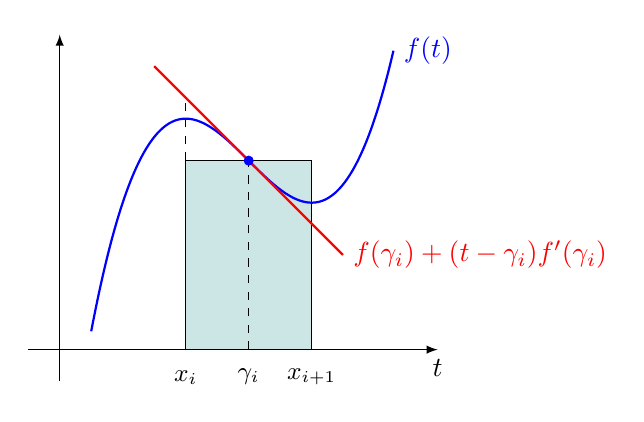
\begin{tikzpicture}[scale=0.8,declare function={f(\x)=((1/3)*(\x)^(3)-3*(\x)^(2)+8*\x-3;}, declare function={g(\x)=-\x+6;},]
\coordinate (xm) at (3,{f(3)});

\draw[fill=teal!20!white] (2,0) rectangle (4,{f(3)});

\draw[dashed] (3, 0) -- (3,{f(3)});
\draw[dashed] (2, {f(3)}) -- (2,{g(2)});

\draw [-latex] (-0.5,0) -- (6,0) node (xaxis) [below] {$t$};
\draw [-latex] (0,-0.5) -- (0,5);
% \foreach \x/\xtext in {1/a=x_0 ,2/x_1, 3/x_2 , 4/x_3 , 5/b=x_4}
\draw[xshift=2 cm] node[below=2pt,fill=white,font=\small, anchor=south, yshift=-5mm] {$x_i$};
\draw[xshift=3 cm] node[below=2pt,fill=white,font=\small, anchor=south, yshift=-5mm] {$\gamma_i$};
\draw[xshift=4 cm] node[below=2pt,fill=white,font=\small, anchor=south, yshift=-5mm] {$x_{i+1}$};
\draw[domain=.5:5.3,samples=200,variable=\x,blue,thick] plot ({\x},{f(\x)}) node[right] {$f(t)$};  
\draw[domain=1.5:4.5,samples=200,variable=\x,red,thick] plot ({\x},{g(\x)}) node[right] {$f(\gamma_i) + (t - \gamma_i) f'(\gamma_i)$}; 
% \foreach \n in {0,1,2,3}
\draw[blue,fill=blue] (xm) circle (2pt) node[font=\normalsize] {$ $};    
% \draw[latex-latex] (2,1)--(3,1) node[midway, anchor=south] {$\frac{b-a}{p}$};      
\end{tikzpicture}